% --------------------------------------
% Document Class
% --------------------------------------
\documentclass[a4paper,11pt]{article}
% --------------------------------------



% --------------------------------------
% Use Package
% --------------------------------------


\usepackage[francais]{babel}
%\usepackage{ucs}
\usepackage[utf8]{inputenc}
\usepackage[T1]{fontenc}

\usepackage{makeidx}
\usepackage{color}
\usepackage{graphicx}
\usepackage{float}
\usepackage[hidelinks]{hyperref} 
\usepackage{geometry}
%\usepackage{lastpage}
%\usepackage{marginnote}
\usepackage{fancyhdr}
%\usepackage{titlesec}
%\usepackage{framed}
\usepackage{amsmath}
\usepackage{empheq}
\usepackage{array}
\usepackage{multicol}
%\usepackage{adjustbox}

% insert code
\usepackage{listings}

% define our color
\usepackage{xcolor}

% code color
\definecolor{ligthyellow}{RGB}{250,247,220}
\definecolor{darkblue}{RGB}{5,10,85}
\definecolor{ligthblue}{RGB}{1,147,128}
\definecolor{darkgreen}{RGB}{8,120,51}
\definecolor{darkred}{RGB}{160,0,0}

% other color
\definecolor{ivi}{RGB}{141,107,185}


\lstset{
    language=Scilab,
    captionpos=b,
    extendedchars=true,
    frame=lines,
    numbers=left,
    numberstyle=\tiny,
    numbersep=5pt,
    keepspaces=true,
    breaklines=true,
    showspaces=false,
    showstringspaces=false,
    breakatwhitespace=false,
    stepnumber=1,
    showtabs=false,
    tabsize=3,
    basicstyle=\small\ttfamily,
    backgroundcolor=\color{ligthyellow},
    keywordstyle=\color{ligthblue},
    morekeywords={include, printf, uchar},
    identifierstyle=\color{darkblue},
    commentstyle=\color{darkgreen},
    stringstyle=\color{darkred},
}


% --------------------------------------



% --------------------------------------
% Page setting
% --------------------------------------
%\pagestyle{empty}
\setlength{\headheight}{15pt}

\setcounter{secnumdepth}{3}
\setcounter{tocdepth}{2}

\makeatletter
\@addtoreset{chapter}{part}
\makeatother 

\hypersetup{         % parametrage des hyperliens
  colorlinks=true,      % colorise les liens
  breaklinks=true,      % permet les retours à la ligne pour les liens trop longs
  urlcolor= blue,       % couleur des hyperliens
  linkcolor= black,     % couleur des liens internes aux documents (index, figures, tableaux, equations,...)
  citecolor= green      % couleur des liens vers les references bibliographiques
}

% --------------------------------------

% --------------------------------------
% Information
% --------------------------------------
\title{Compte-rendu TP6 Rdf : Classification supervisée par analyse discriminante}
\author{Elliot VANEGUE et Gaëtan DEFLANDRE}
% --------------------------------------

\definecolor{myColor}{rgb}{0.5, 0.1, 0.75}

% --------------------------------------
% Begin content
% --------------------------------------
\begin{document}

% Set language to english
  \selectlanguage{francais}

  % Start the page counting
  \pagenumbering{arabic}

  \maketitle
  
  \mbox{}
  \newpage
  \clearpage
  
  \section*{Introduction}
  Lors de ce TP, nous allons utiliser une analyse discriminante dans
  le but de classifier les données d'une image. Pour cela, nous allons
  utiliser les données présentent dans un fichier Rdata afin de
  calculer des moyennes de covariance et effectuer des analyses
  linéaires. Nous séparerons ainsi les données en plusieurs classes.

  \section{Classification de données gaussiennes}
  \subsection{Affichage des données d'apprentissage et de test}
  Les données d'apprentissage sont des données qui vont nous permettre
  de diviser les points d'une image en un nombre K d'ensemble. Pour
  cela chaque point possède une couleur qui représente l'ensemble
  auquel il appartient.  Ce qui nous donne le graphe suivant pour les
  données d'apprentissage :
  
  \begin{figure}[H]
   \centering
   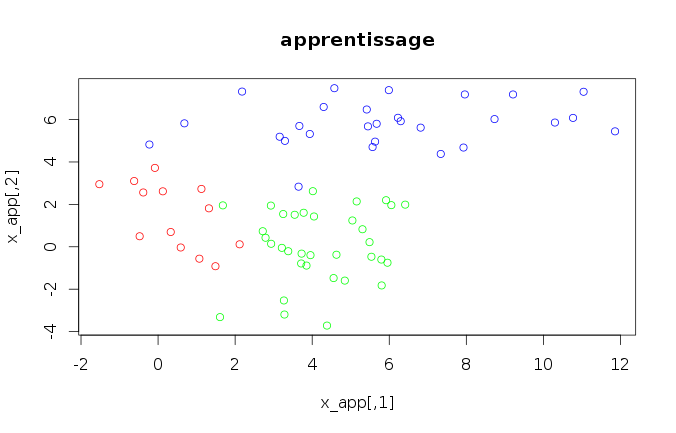
\includegraphics[width=10cm]{ensemble_apprentissage.png}
   \caption{Graphe d'apprentissage}
  \end{figure}

  Nous pouvons également afficher les données de test afin de voir les
  différences avec les données d'apprentissage.
  \newpage
  \begin{figure}[H]
   \centering
   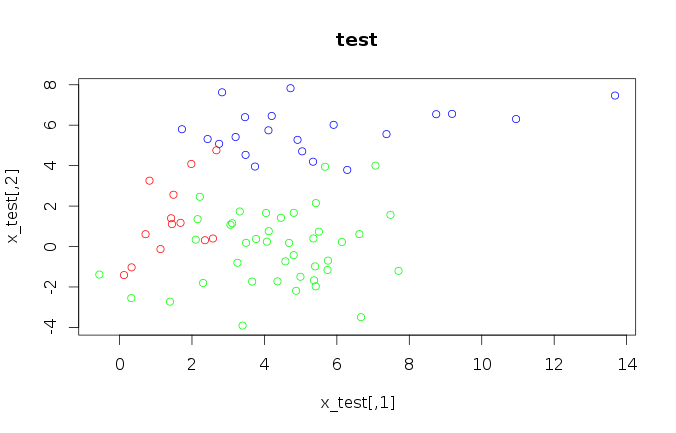
\includegraphics[width=10cm]{ensemble_test.png}
   \caption{Graphe de test}
  \end{figure}
   
  \subsection{Estimation des moyennes et co-variance des observations d'apprentissage}
  Nous avons ensuite estimé une moyenne des données d'apprentissage
  sur les attributs de chaque classe afin de les comparer aux moyennes
  des données test. Pour cela, nous appliquons la macro R suivante sur
  chaque classe :
  
  \begin{lstlisting}[caption=Estimation de la moyenne pour la classe d'apprentissage 1]
  M1<-seq(1,2)
  M1[1] = mean(x_app[classe_app==1,1])
  M1[2] = mean(x_app[classe_app==1,2])
  \end{lstlisting}
  \ \\
  Ce qui nous a donné les valeurs suivantes :\\
  
  \begin{center}
    \begin{tabular}{|c|c|c|c|c|}
    \hline
    \multicolumn{3}{|c|}{apprentissage} & \multicolumn{2}{c|}{test}\\
    \hline
    classe & attribut 1 & attribut 2 & attribut 1 & attribut 2\\
    \hline
    1 & 0.39 & 1.48 & 1.44 & 1.31\\
    \hline
    2 & 5.97 & 5.81 & 5.43 & 5.74\\
    \hline
    3 & 4.19 & 0.05 & 4.34 & -0.10\\
    \hline
    \end{tabular}
  \end{center}
  
  Nous pouvons voir que les moyennes des données d'apprentissage sont
  assez proches des moyennes des données de test, mais présentent
  quelques différences. Nous allons donc effectuer une analyse
  discriminante sur les données, afin de les segmenter de manière
  automatique.\\
  
  Par la suite, nous avons calculé les matrices de covariance de
  chaque classe afin de calculer l'écart qu'il y a entre les deux
  attributs de chaque valeur. Pour cela, nous avons utilisé la macro
  suivante :
  
  \begin{lstlisting}[caption=Calcul de covariance de la classe d'apprentissage 1]
  Sigma1[i,j]=cov(as.vector(x_app[classe_app==1,i]), as.vector(x_app[classe_app==1,j]))
  \end{lstlisting}
  
  Ce qui nous donne les matrices de covariance suivante : 
  \begin{center}
    \begin{tabular}{|c|c|}
    \hline
    classe & matrice de covariance\\
    \hline
    1 & 
    $\begin{pmatrix}
     1.03 & -0.93\\
     -0.93 & 2.46
    \end{pmatrix}$\\
    \hline
    2 & 
    $\begin{pmatrix}
     9.15 & 0.73\\
     0.73 & 1.16
    \end{pmatrix}$\\
    \hline
    3 & 
    $\begin{pmatrix}
     1.59 & 0.29\\
     0.29 & 2.91
    \end{pmatrix}$\\
    \hline
    \end{tabular}
  \end{center}
  
  Nous remarquons que les valeurs de l'écart-type pour les deux attributs sont présentes dans la matrice
  de covariance :
  \begin{itemize}
   \item la valeur, en haut à gauche, représente l'écart-type pour l'attribut 1.
   \item la valeur, en bas à droite, représente l'écart-type pour l'attribut 2.
  \end{itemize}
  

  \subsection{Analyse linéaire discriminante (LDA)}
  
  Nous avons ensuite appliqué une analyse linéaire discriminante sur
  les données afin de les classifier. Grâce à une macro, nous avons pu
  déterminer que le taux de bonne classification des données est de
  84\%. Ce qui nous permet d'obtenir la LDA suivante :\\

  \begin{figure}[H]
   \centering
   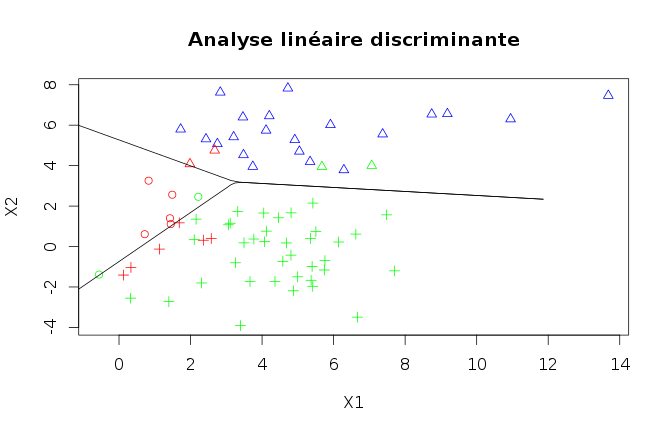
\includegraphics[width=10cm]{lineaire_discri.png}
   \caption{Graphe de l'analyse linéaire discriminante des données test}
  \end{figure}

  Nous représentons les points par deux caractéristiques :
  \begin{itemize}
   \item la couleur correspond à la classe à laquel devrait appartenir la donnée.
   \item la forme correspond à la classe à laquel appartient la donnée avec nos calculs.
  \end{itemize}
  
  
  \subsection{Analyse quadratique discriminante (QDA)}
  
  Nous avons appliqué une seconde analyse discriminante pour
  déterminer les classes des données test.  Nous avons utilisé la même
  macro que précédemment, mais cette fois en passant par une analyse
  quadratique, ce qui nous a donné le résultat suivant :\\
  
  \begin{figure}[H]
   \centering
   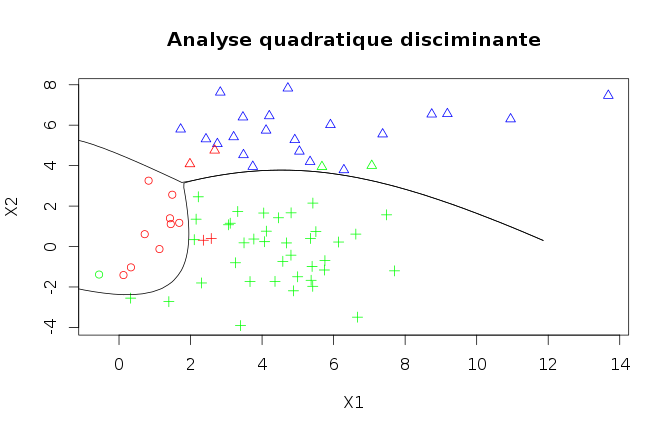
\includegraphics[width=10cm]{quadratique.png}
   \caption{Graphe de l'analyse quadratique discriminante des données test}
  \end{figure}
  
  On voit que les séparations des classes, contrairement à l'analyse
  linéaire, sont courbes et donc englobe mieux les données de chaque
  classe. C'est pourquoi il semble qu'il y ait moins d'erreurs sur la
  classification de la classe rouge.\\
  
  Par cette méthode, nous obtenons un taux de bonne classification de
  90\% pour les données test.  On peut voir que pour ces données, la
  meilleure analyse est la quadratique, car elle a un meilleur taux de
  bonne classification.
  
  \section{Classification de données réelles : Iris}
  
  \subsection{Analyse linéaire discriminante (LDA)}
  
  Nous allons maintenant appliquer l'analyse linéaire discriminante
  sur des données réelles afin de voir si cette méthode est aussi
  efficace quel que soit le type de données. Nous obtenons pour les
  données de l'Iris un taux de bonne classification de 97\%, ce qui
  est supérieur à des données gaussiennes. Nous avons alors la
  classification suivante :\\
  
  \newpage
  \begin{figure}[H]
   \centering
   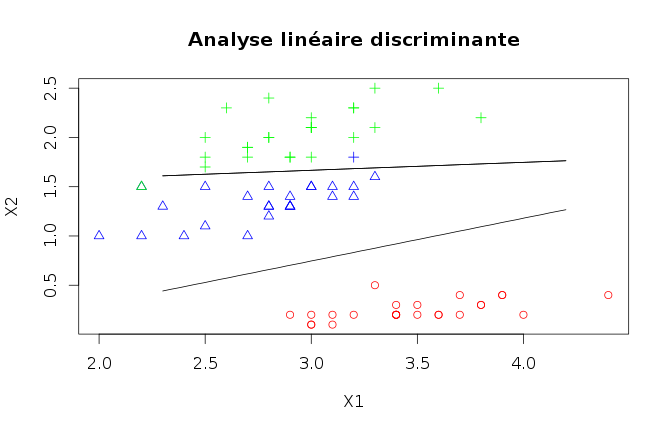
\includegraphics[width=10cm]{iris_lineaire.png}
   \caption{Graphe de l'analyse linéaire discriminante des données test de l'Iris}
  \end{figure}
  
  \subsection{Analyse quadratique discriminante (QDA)}
  
  Nous avons également utilisé une analyse quadratique, ce qui nous a
  donné un taux de bonne classification de 96\%. On remarque que cette
  fois, sur des données réelles, l'analyse linéaire est meilleure que
  l'analyse quadratique.
  
  \begin{figure}[H]
   \centering
   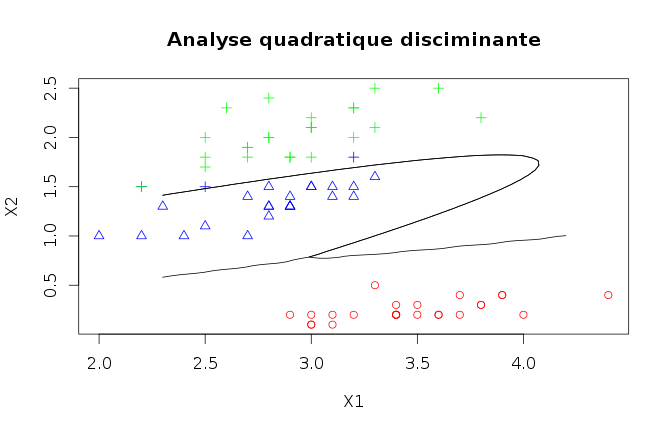
\includegraphics[width=10cm]{iris_quadratique.png}
   \caption{Graphe de l'analyse quadratique discriminante des données test de l'Iris}
  \end{figure}
  
  On remarque une fois encore que l'analyse quadratique possède des
  séparations courbes, mais cela n'intervient pas sur les données, car
  celle-ci se mélange très peu.
  
  %TODO inversion des données
  %Sa il faudrait que tu essaye parce que moi j'obtient un taux de bonne classifiation
  %en linéaire qui est le même que le quadratique sans inversion.
  
  \section*{Conclusion}
  Nous avons donc vu lors de ce TP, comment effectuer des analyses
  discriminantes dans le but de classer les données d'une
  image. Cependant, cette méthode nécessite d'avoir une base de
  connaissance % pour pas dire données d'apprentissage 
  pour effectuer
  la séparation des données. Nous avons également vu que l'analyse
  linéaire et quadratique sont des méthodes très efficaces, mais qui
  sont plus performantes sur certain type de donnée.
\end{document}  
